%this file is the analysis report of POO project
%a % comment anything after % until the end of the line
%minimum references to begin our article
\documentclass[12pt]{article}

\usepackage[french]{babel}
\usepackage[utf8]{inputenc}
\usepackage[T1]{fontenc}
\usepackage{graphicx}
\usepackage{fancyhdr}
\usepackage{hyperref}
%\usepackage{float}
%\usepackage{amsmath}
%\usepackage[margin=1in]{geometry}
%\usepackage{indentfirst}
%\usepackage{titlesec}

\newcommand{\sectionbreak}{\clearpage}
\pagestyle{fancy}
%\cfoot{Rapport de présentation projet POO}
% the last extension makes it possible to add images
%presentation of the document
\title{Projet Modéliation et Programmation Orientée Objet\smallbreak Rapport d'analyse du jeu et de conception du logiciel}
\author{Julien \textsc{Bouvet}, Mikail \textsc{Demirdelen} \\}
\date{08/11/2014}
\setlength\parindent{15pt}
\begin{document}
\maketitle
\newpage
\begin{abstract}
A-t-on besoin d'un abstract ?
\end{abstract}
\newpage
%to add a table of contents
\tableofcontents
\newpage
\section{Introduction}

Dans le cadre du Projet MOO/MOO/COO, bla bla, on va faire un jeu qui roxxe sa mère (JE SAVAIS PAS COMMENT COMMENCER ><) \newline \newline
Le principe de ce projet est d'avoir une première aproche de la programmation et modélisation orientée objet à travers un logiciel relativement complexe. Nous devons donc implémenter un jeu de stratégie au tour par tour et pour ce faire nous allons passer par différentes phases de conception.
\begin{itemize}
  \item Analyse du jeu : Nous devrons comprendre et assimiler le fonctionnement du jeu afin de concevoir son fonctionnement logiciel. De plus, nous allons devoir en détailler les règles.
  \item Analyse de la structure du logiciel :  A l'aide de différents diagrammes, nous allons pouvoir définir conceptuellement plusieurs classes, leurs différentes relations et interactions. De plus, nous devrons utiliser des patrons de conception pour rendre plus générique la modélation de notre logiciel.
  \item Implémentation du jeu : Nous allons développer concrètement le jeu dans le langage C\#, nous permettant d'appliquer les principes de programmation orientée objet.
\end{itemize}
\newpage

\section{Présentation du jeu}
Le jeu est un jeu de stratégie au tour dans lequel chaque joueur contrôle un peuple. Le joueur doit gérer des unités sur une carte afin d'obtenir le plus de points possible après un certain nombre de tours de jeu.
\subsection{Règles de base}
 Afin d'avoir le plus de points possible, le commence avec des unités placées sur une même case de la carte. Il a ensuite le choix de les répartir comme bon lui semble.Chaque case contrôlée rapport un point. Il est possible d'utiliser certains bonus pour augmenter la valeur d'une case. A CONTINUER.

\subsection{Les peuples}
Il existe trois peuples : les Elfs, les Orcs et les Nains. Chaque peuple a ses propres caractéristiques très différentes influant les différentes stratégies de jeu. Un joueur ne peut choisir qu'un seul peuple.
\subsubsection{Elf}
Les mecs de la forêt ma gueule
\subsubsection{Orc}
Les mecs de la plaine ma gueule
\subsubsection{Nain}
Les mecs de la montagne ma gueule

\subsection{La Carte du monde}
La carte du monde se compose de cases hexagonales. Il existe différents types de cases. A CONTINUER.

\subsubsection{Types de cartes}
Il existe 3 types de cartes :
\begin{itemize}
  \item Démo : 2 joueurs, 5 cases x 5 cases, 4 unités par joueur.
  \item Petite : 2 joueurs, 10 cases x 10 cases, 6 unités par joueur.
  \item Normale :  2 joueurs, 15 cases x 15 cases, 8 unités par joueur.
\end{itemize}

\subsection{Les Combats}
BLA BLA

\subsection{Début de partie}
BLA BLA

\subsection{Déroulement d'un tour}
\newpage

\section{Présentation du logiciel}

\subsection{Architecture générale}
Notre première analyse porta sur l'architecture générale du logiciel. Nous avons ainsi conçu un diagramme de classe correspondant à notre vision du jeu, représenté à la figure \ref{classe}

\begin{figure}[!h] 
\centerline{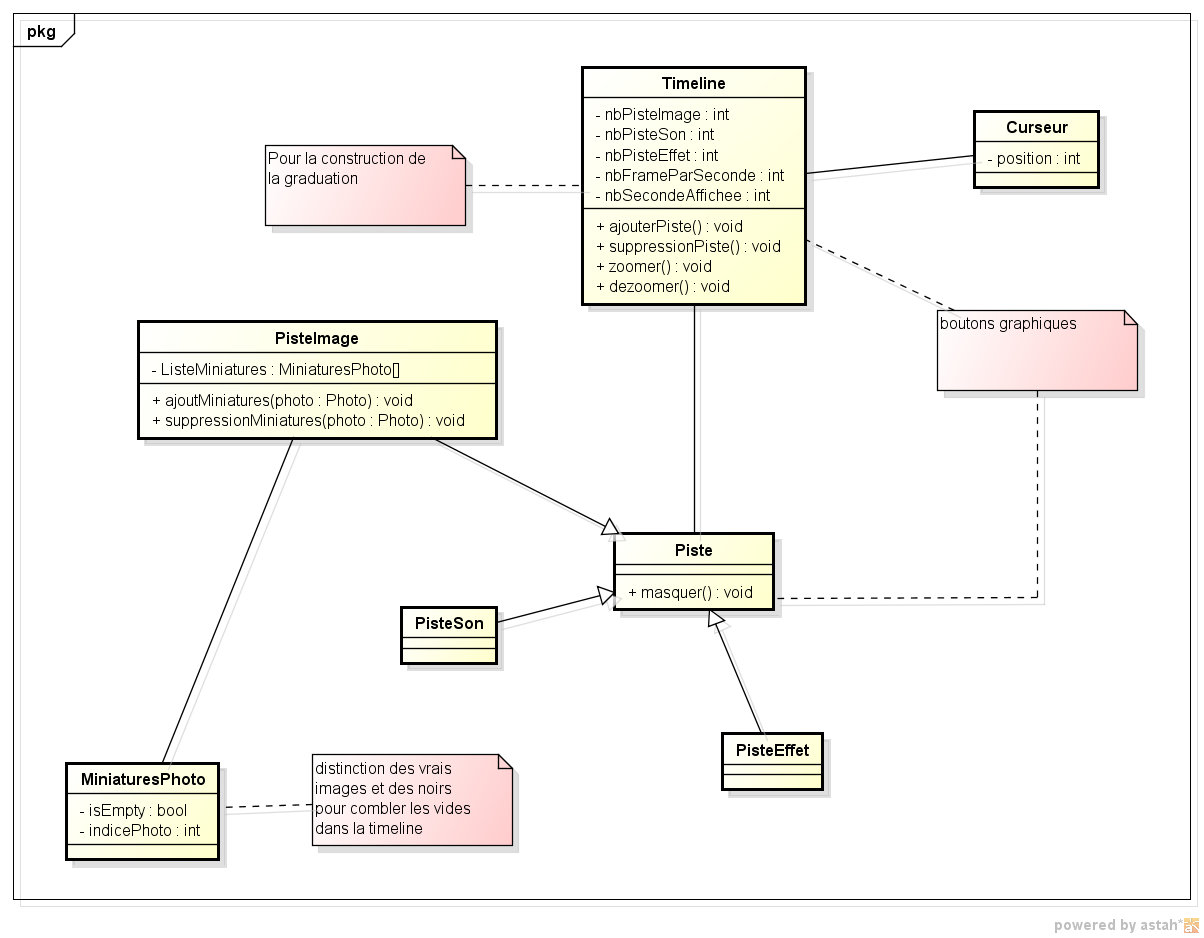
\includegraphics[scale=0.60]{diag_class_ex.png}}
   \caption{\label{étiquette} Diagramme de classe du logiciel}
\label{classe}
\end{figure}

Sur ce diagramme, nous avons 5 principaux acteurs.
\begin{itemize}
  \item Le Jeu, ou Game, qui représente la partie du jeu. Il fait le lien entre le Joueur (Player) et le Plateau (Board). 
  \item Le Joueur, ou Player, est la classe représentant, comme son nom l'indique, le joueur. C'est lui qui intéragira avec la vue du plateau, et qui donnera des ordres à ses Unités.
  \item Le Plateau, ou Board, contient les cases sur lequel le jeu évolue. Il contient aussi les différentes unités en jeu. Cela permet un accès plus rapide pour le traitement de certaines actions.
  \item Les Cases, ou Tiles, sont les cases, au sens individuel du terme, contenues sur le Plateau. Elle possèdent les Unités qui se trouvent sur elle. Elle hérite 4 autres classes, chacune correspondant au type de terrain associé : Plaine, Désert, Forêt, Montagne.
  \item Les Unités, ou Units, sont les personnages évoluant sur la carte. Les différents peuple sont ici défini comme héritant la classe Unité. Ainsi, on peut surcharger des fonctions, comme le déplacement ou l'attaque, en fonction du peuple de l'Unité : Elf, Orc ou Nain.
\end{itemize}

\subsection{Cas d'utilisations}
Après avoir pensé au logiciel en tant que tel, nous avons réfléchi sur l'interaction que le logiciel aurait avec l'utilisateur. Sur la figure \ref{casdut1}, on peut voir le fonctionnement global du logiciel. Sur la figure \ref{casdut2}, on BLA BLA BLA.

\begin{figure}[!h] 
\centerline{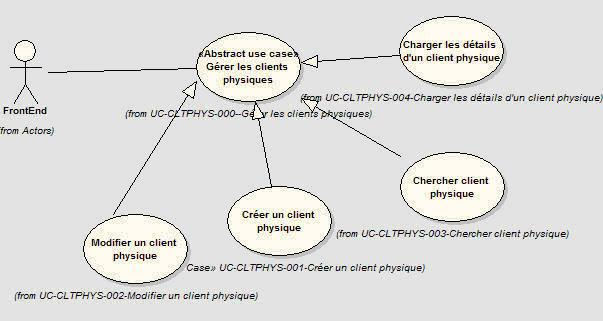
\includegraphics[scale=0.60]{diag_cas_dut_ex.jpeg}}
   \caption{\label{étiquette} Diagramme de cas d'utilisations global}
\label{casdut1}
\end{figure}

\begin{figure}[!h] 
\centerline{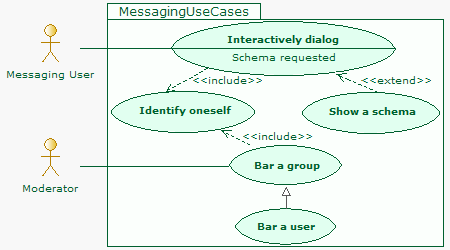
\includegraphics[scale=0.60]{diag_cas_dut2_ex.jpeg}}
   \caption{\label{étiquette} Diagramme de cas d'utilisations spécifique}
\label{casdut2}
\end{figure}

\subsection{Déroulement globale d'une partie jusqu'à la victoire d'un joueur}
Pour les diagrammes de séquence et d'activité
\subsection{Déroulement d'un tour pour un joueur}
Pour les diagrammes de séquence et d'activité

\subsection{Cycle de vie d'une unité}
Pour le diagramme, ô combien inutile :p, d'états-transitions
\newpage

\section{Conclusion}

\newpage

\bibliography{bibliography}
\bibliographystyle{plain}
\end{document}